\titre{Définition :} On appelle ensembles disjoints une collection $S=S_1,\ldots,S_n$ d'ensembles deux à deux disjoints. On va effectuer des opérations sur ces ensembles (ex : union, déterminer si un élément est dans un des ensembles, si deux ensembles sont contenus dans un autre ensemble etc). \\

\titre{Utilisations classiques :}
\begin{itemize}
	\item Calculer les composantes connexes d'un graphe (fermeture transitive de la relation d'adjacence)
	\item Calculer des classes d'équivalence de façon générale
	\item Déterminer si un graphe contient un cycle (algo de Kruskal)
\end{itemize}

\titre{Opérations sur ces structures :} Les éléments des ensembles sont appelés "objets" (pointeur vers un élément avec des informations) :
\begin{itemize}
	\item Creer-ensemble(x:objet) : Créer un ensemble réduit au singleton x
	\item Trouver-ensemble(x:objet) : retourne un objet qui est le représentant de tous les objets du meme ensemble.
	\item Union(x,y:objet) avec x $\neq$ y et Trouver-ensemble(x) $\neq$ Trouver-ensemble(y). Attribue un nouveau représentant et réalise l'union.
	\item On pourrait rejouter des opérations de division d'ensemble mais ça ne présente aucune difficulté.
\end{itemize}

\titre{Exemple :} Calcul de composantes connexes. On voudrait savoir si deux sommets d'un graphe sont dans la même composante connexe (ie existe-t-il un chemin entre ces deux sommets), combien il y a de composantes connexes dans le graphe, etc. \\
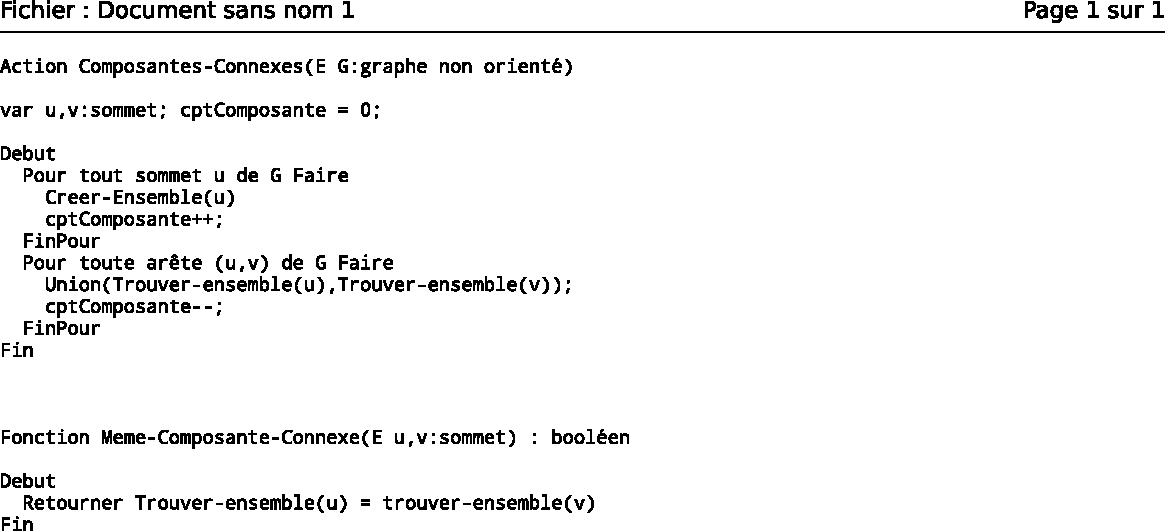
\includegraphics{Images/fig3.pdf} \\
Le cout est donc n Creer-ensemble + 2m Trouver-ensemble + min(n,m) Unions \\

\titre{Représentation par listes chaînées :} On représente chaque ensemble par une liste chainée enrichie. 
\begin{itemize}
	\item Creer-ensemble est en $\theta(1)$
	\item Trouver-ensemble est en $\theta(1)$
	\item Union : pour pouvoir fusionner la plus petite à la grande, il nous faut rajouter une donnée : le nombre d'éléments de chaque liste. Cela permet de réduire la complexité au point où $n$ creer-ensemble et $m$ opérations quelconques, alors le coût amorti total est de $\theta(m+n\mathrm{ln}n)$ On le démontre avec la méthode des agrégats. 
\end{itemize}

\titre{Preuve :} \\
La complexité totale correspond au nombre de fois où le lien "représentant" est modifié. \\
Pour un objet x, son représentant est modifié lors d'une union où x était dans le plus petit ensemble. \\
Au début, x est dans un ensemble à un élément. \\
Si son représentant est modifié une fois alors il est dans un ensemble à au moins 2 éléments.\\
Si son représentant est modifié une deuxième fois alors il est dans un ensemble à au moins 4 éléments.\\
La taille double à chaque fois, d'où le $\mathrm{ln}n$ \\
Et il y a n éléments, donc on a au maximum $n\mathrm{ln}n$ changements de représentants.\\

\titre{Représentation par forêt :} Un ensemble a un représentant unique qui va être la racine d'un arbre. Tous les éléments d'un ensemble vont être dans le même arbre, et on a un arbre par ensemble. La forêt est l'union disjointe des arbres. Chaque élément, en plus de sa valeur, stockera un pointeur vers son père dans l'arbre (ou lui même si c'est la racine), ainsi qu'u entier appelé rang. \\

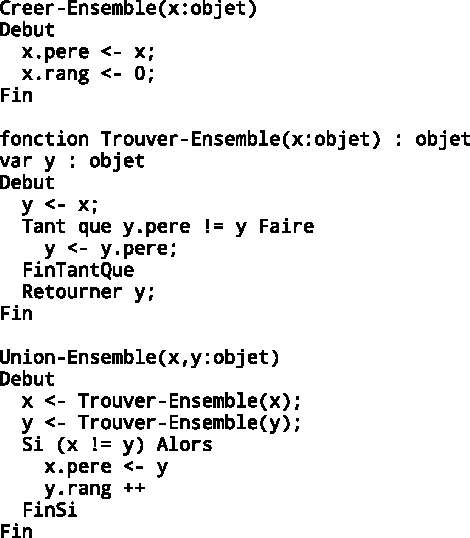
\includegraphics{Images/fig4.pdf}\\

\titre{Idées :}
\begin{itemize}
	\item Union par rang : on connecte l'arbre qui a le plus petit rang à l'autre. \\
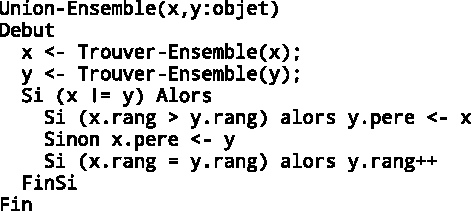
\includegraphics{Images/fig5.pdf}\\
	\item Compression de chemin : On profite d'un appel à Trouver-Ensemble pour mettre à jour tous les pères sur le chemin de l'objet jusqu'à sa racine.\\
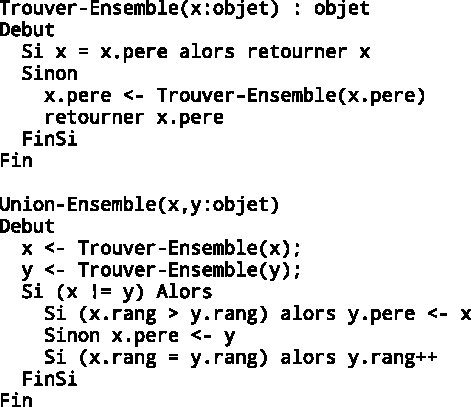
\includegraphics{Images/fig6.pdf}\\
\end{itemize}

\titre{Théorème de Tarjan (1975) :} Si on utilise ce type de structure Union-Find avec union par rang et compression de chemin, alors une séquence arbitraire de m opérations Creer-Ensemble, Trouver-Ensemble et Union-Ensemble prend un temps en $\theta(m\alpha(n))$ où $\alpha(n)$ croit très lentement (impossible de représenter en mémoire un entier $n$ qui rend $\alpha(n) \leq 4$). \\

\titre{Explication :} $\alpha$ est l'inverse d'une fonction qui croit très vite : $A_k(1)$ ... $\alpha(n)$ = plus petit $k$ tel que $A_k(1)\geq n$. Avec $A_k$ la fonction de Ackermann : qui à $k\geq 0, j \geq 1$ associe $A_k(j) = \left\{ \begin{array}{l}
	j+1 \mathrm{si} k = 0
	A_{k-1}(A_{k-1}( \ldots A_{k-1}(j)))) \mathrm{sinon} \end{array} \right.$

$$
\begin{array}{c|cccccc}
	j & 1 & 2 & 3 & 4 & 5 & 6 \\ \hline
A_0(j) & 2 & 3 & 4 & 5 & 6 & 7  \\ \hline
A_1(j) & 3 & 5 & 7 & 9 & 1 & 13  \\ \hline
A_2(j) & 7 & 23 & 63 & \ldots \\ \hline
A_3(j) & 2047 & >2^{2^{27}} & \ldots \\ \hline
A_4(j) & >> 2^{2048} & \ldots \\ \hline
\end{array}
$$

\titre{Conclusion :} Union-Find peut être considéré comme linéaire.\\

\titre{Exercice :} Quel est le rang max que l'on peut obtenir avec 7 unions sur 8 éléments ? Réponse : 3 (en réalité pour faire un rang $k$ il faut $2^k$ éléments. On voit donc qu'il y a majoration par $m\ln n$. \\

\titre{Exercice :} Si on fait trouver-Ensemble sur un sommet de profondeur $k$, quelle est la variation de la somme des profondeurs de l'arbre ? \\

